

\documentclass[a4paper]{scrartcl}
%\documentclass[class=article,a4paper,11pt,twoside]{beamer}

\usepackage[utf8]{inputenc}
\usepackage[english]{babel}
\usepackage{lmodern} 
\usepackage[T1]{fontenc}
\usepackage{booktabs}
\usepackage{multirow}
\usepackage{wrapfig}


% PAKETE
\usepackage{siunitx}
\usepackage{graphicx}
\usepackage{placeins}
\usepackage{longtable}
\usepackage{enumitem}
\usepackage{bbm}
%\usepackage{sidecap}


\usepackage{amssymb} % math symbols
\usepackage{amsmath} % ams
\usepackage{amsfonts} % mathmatical fonts

% caption indenting
 \usepackage[format=plain,indention=0em,labelfont=bf,margin=1em]{caption} 
 \usepackage{subfig} %subfigures ^^
\usepackage[protrusion=true,expansion=true]{microtype} % denser font, "-" behind line
\usepackage{esint} % nicer double and triple integrals
\usepackage{fancyhdr} % fancy headers
\usepackage[colorlinks=true,linkcolor=black,citecolor=black,filecolor=black,urlcolor=black]{hyperref}

\usepackage{fullpage}

% EINSTELLUNGEN
\sisetup{seperr,repeatunits=false}
\numberwithin{equation}{section}
\numberwithin{figure}{section}
\numberwithin{table}{section}

% EIGENE FUNKTIONEN
\newcommand{\re}{\operatorname{Re}}
\newcommand{\im}{\operatorname{Im}}
\newcommand{\gquote}[1]{\glqq #1 \grqq}

\newcommand{\eq}[2]{\begin{equation}#1\label{#2}\end{equation}}
\newcommand{\eqand}[0]{\hspace{.25cm} \bigwedge \hspace{.25cm}}
\newcommand{\grafik}[2]{\begin{figure}[h]\centering \includegraphics[width=10cm]{#1.eps}  \caption{#2} \label{#1} \end{figure} }
\newcommand{\grafikq}[3]{\begin{figure}[h]\centering \includegraphics[width=10cm]{#1.eps}  \caption[#2]{#3} \label{#1} \end{figure} }
\newcommand{\tbl}[3]{\begin{table}[h]\caption{#1}\label{#2}\begin{center}#3\end{center}\end{table}}
\newcommand{\Abbildung}[1]{\textsl{Abbildung \ref{#1}}}
\newcommand{\AbbildungI}[1]{\textsl{(Abbildung \ref{#1})}}
\newcommand{\Tabelle}[1]{\textsl{Tabelle \ref{#1}}}
\newcommand{\TabelleI}[1]{\textsl{(Tabelle \ref{#1})}}
\newcommand{\Formel}[1]{(\ref{#1})}
\renewcommand{\d}{\mathrm{d}}
\newcommand{\ve}[1]{\mathbf{ #1} }

\newcommand{\ssubsection}[1]{{ \subsection*{\linebreak \centering\bf\underline {#1}}}}
\renewcommand\refname{}

\begin{document}
%\section*{Superconductivity}
\begin{center}
\Huge \bf \sc Superconductivity \\
\large B. Huber \quad C. Wille \\
\small 28.11.2011
\end{center}
\small
\ssubsection{Historical Overview}
Superconductivity was found experimentally in 1911 by H. Kammerlingh Onnes. The liquidation of helium made experiments below $T=4$ K possible. Onnes investigated the electrical resistivity of metals, which was believed to decrease with temperature smoothly as the oscillation of the lattice atoms decline. It was predicted that it reaches a finite value at zero temperature due to impurities of the metal, instead for various materials the rapid decay of resistivity at a certain temperature $T_C$ was detected (figure 1). 

\begin{wrapfigure}{r}{0.3\linewidth}
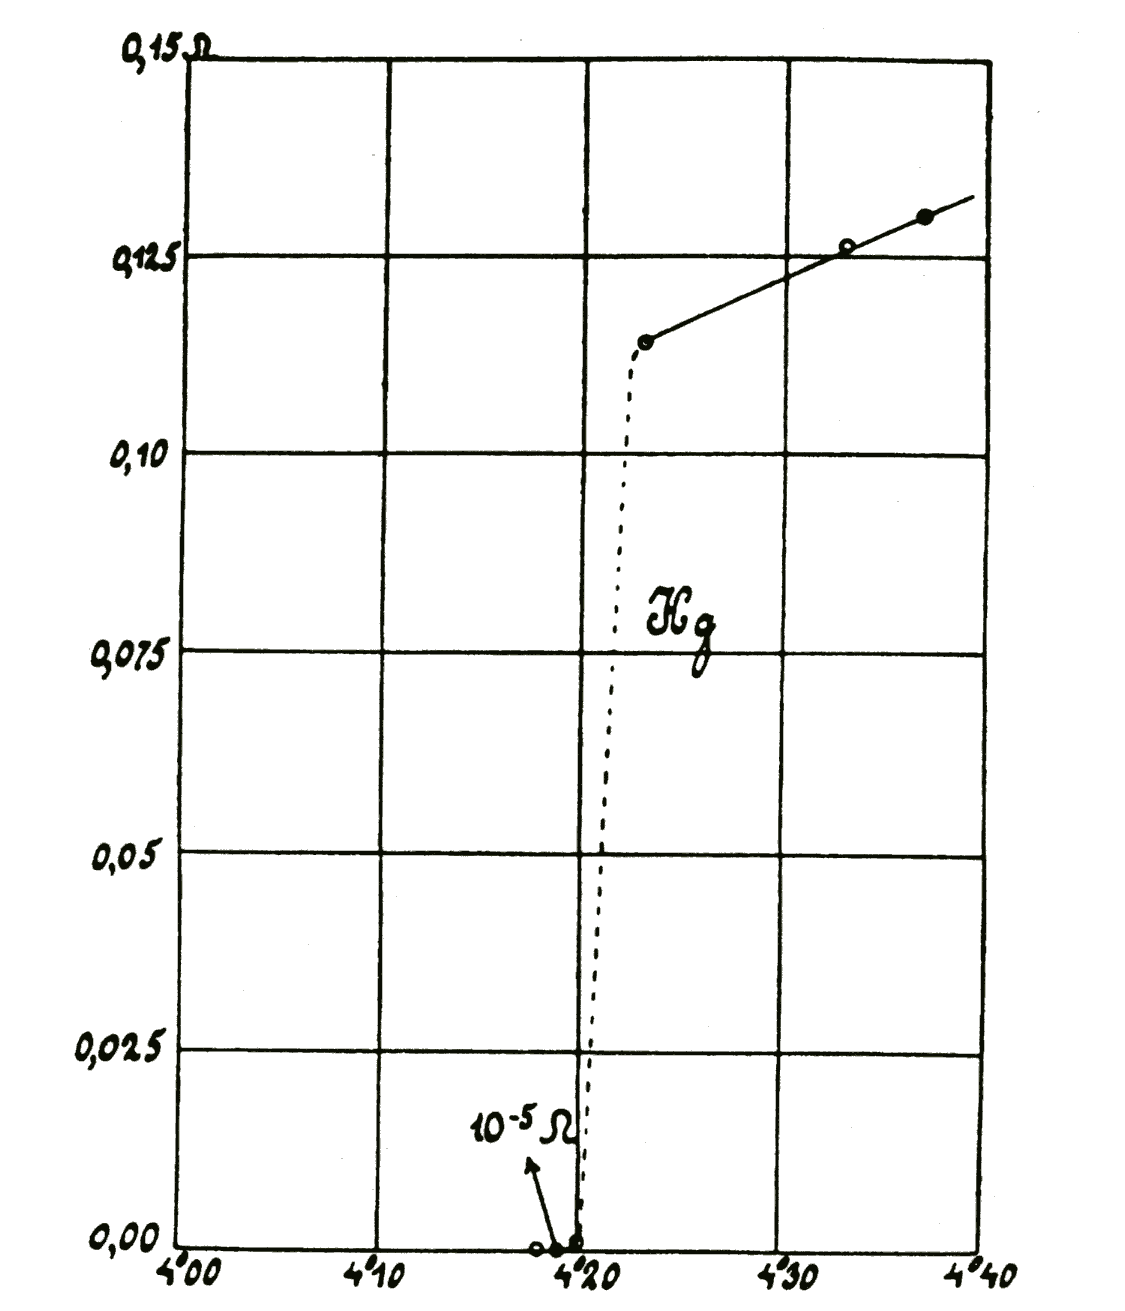
\includegraphics[width=0.3\textwidth]{img/heikemess.png}
\caption*{\textbf{Figure 1: }\small Original Data for Mercury (Onnes, 1911) \cite{buckel}}
\label{fig:onnes}
\end{wrapfigure}

The first phenomenological theory of superconductivity was developed by the brothers F. and H. London in 1935 after the discovery of the Meißner-Ochsenfeld Effect in 1933 and during the 1950s the more elaborate Ginsburg-Landau-Theory was developed. In 1957 Bardeen, Schriefer and Cooper published their famous paper on a microscopic description of superconductivity, the BCS Theory.

\ssubsection{Properties of Superconductors}
The superconducting state is a new phase of matter and therefore has many new characteristics. The most important feature is the loss of electrical resistivity. Furthermore, there are three distinct critical values, which lead to the destruction of perfect conduction. These are critical temperatures, critical magnetic fields and critical electric currents. The destruction of superconductivity by all three cab be explained by the BCS theory and is linked to the binding energy of the Cooper pairs. Further remarkable properties are the quantized magnetic fluxes in certain sample geometries (e.g. rings). The energy gap of superconductors is also a very prominent feature and leads to phenomena such as the Josephson currents, which have great application in very sensitive electronical devices (SQUIDs). 

\ssubsection{Mei\ss ner-Ochsenfeld Effect}
For a hypothetic material, which becomes perfectly conducting below certain magnetic fields and temperatures, it would be possible to create different phase states depending on the path, that is chosen to undergo a phase transition in the T-B-diagram (see figure 2). Activating a magnetic field during the non perfectly conducting phase and cooling down afterwards, should lead to magnetic flux inside the material. However, this is not the case for superconductors. Instead, it is an outstanding property of the superconducting phase, that all magnetic flux is expelled from the interior of the sample. This effect is called the Meißner-Ochsenfeld Effect.

\begin{figure}[!tbh]
\subfloat[][]
	{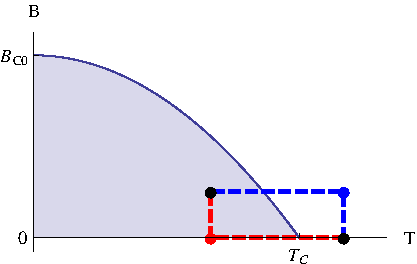
\includegraphics[width=0.3\textwidth]{img/tb6.pdf}}
\subfloat[][]
	{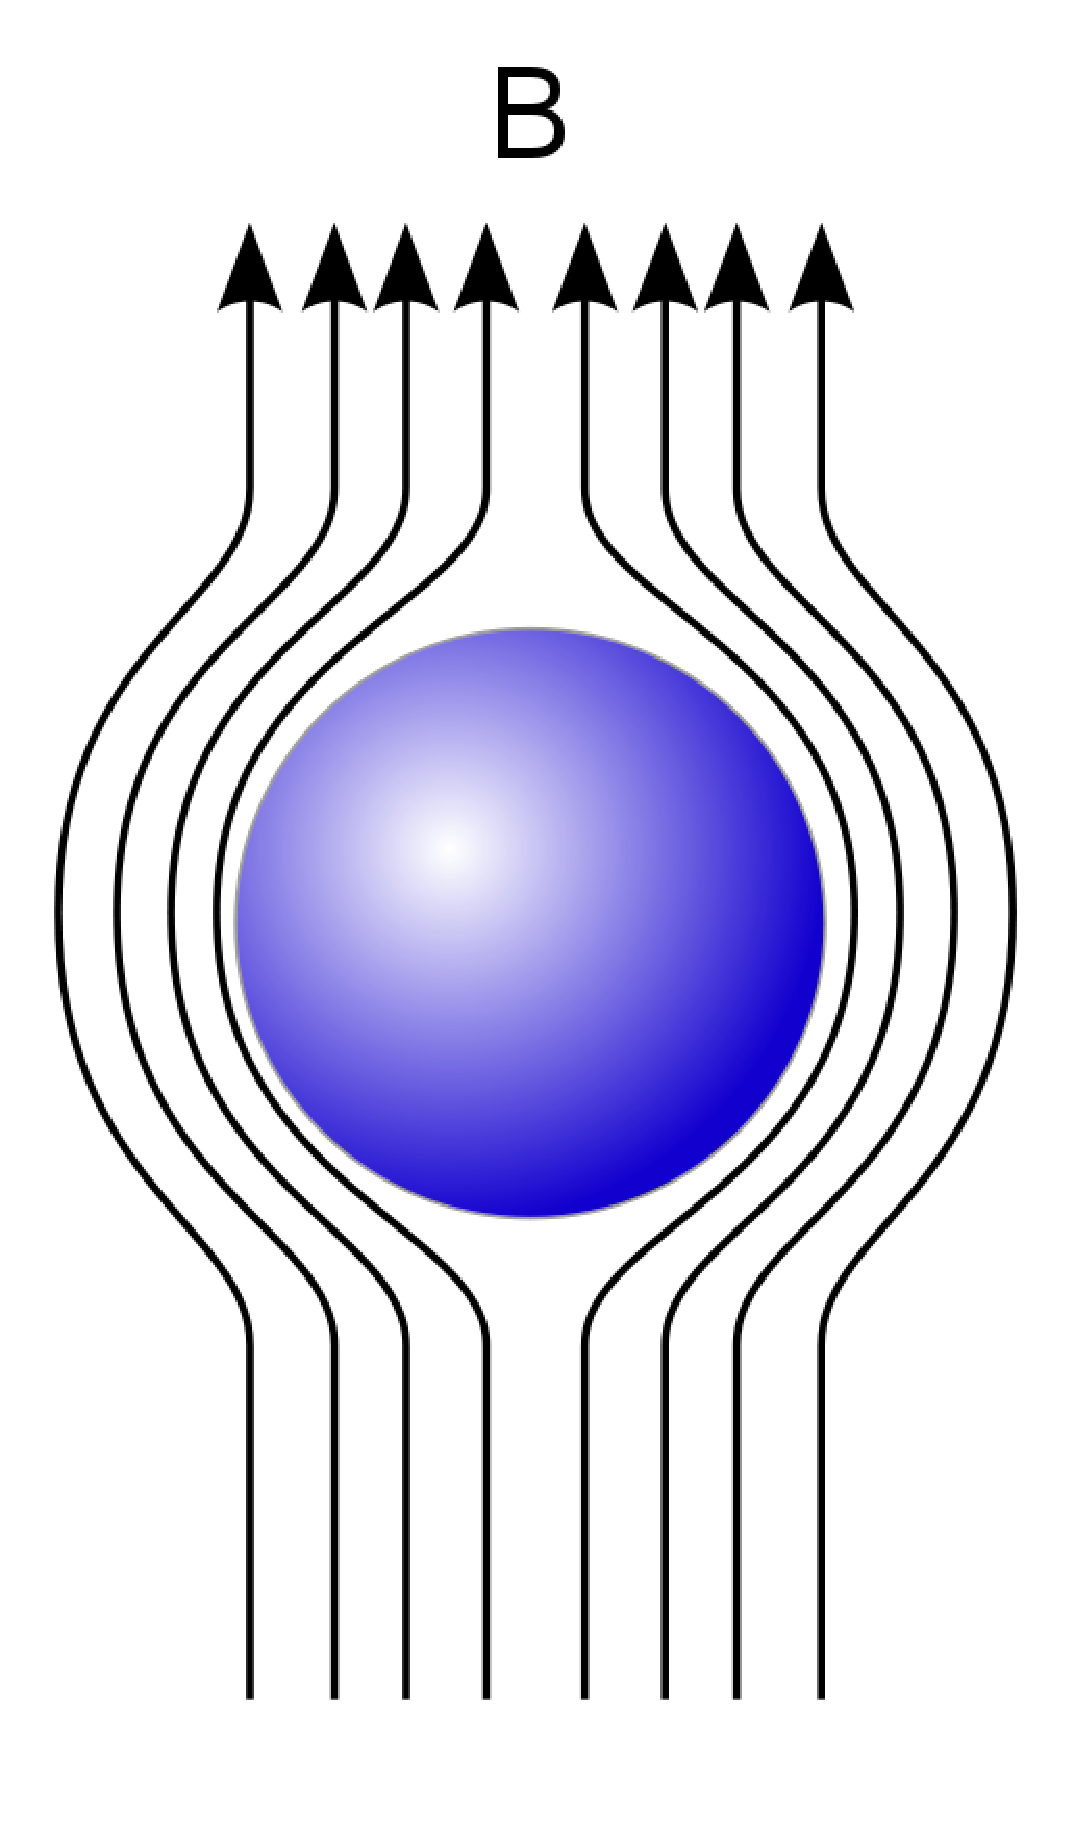
\includegraphics[width=0.15\textwidth]{img/nichdurch.pdf}}
\subfloat[][]
	{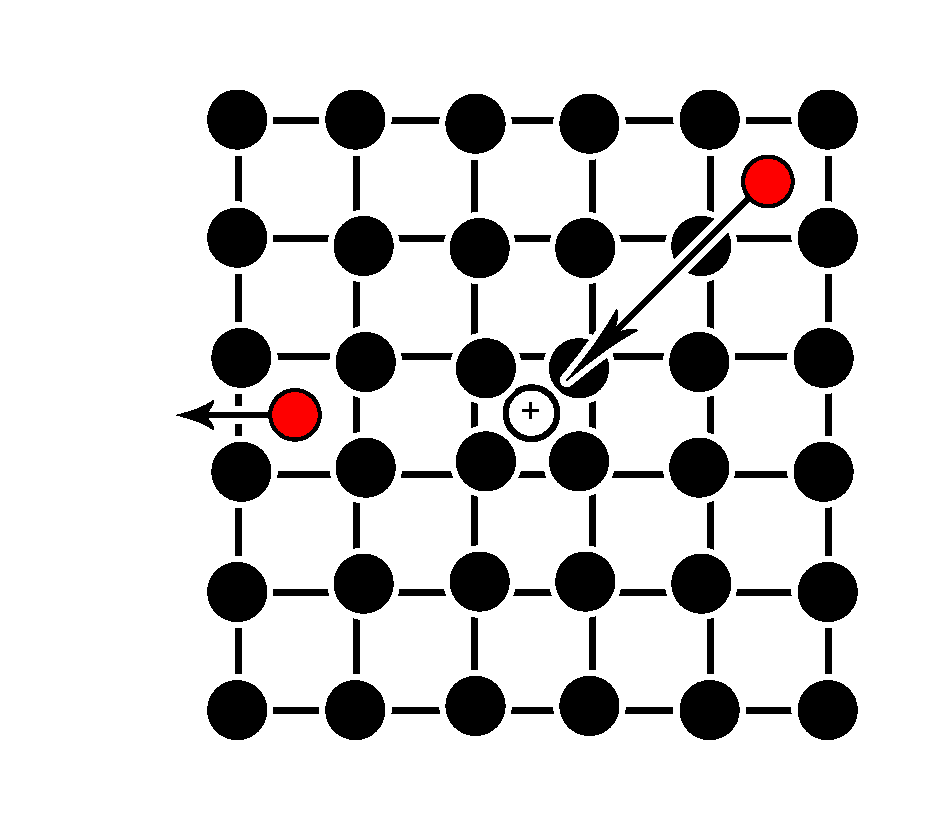
\includegraphics[width=0.3\textwidth]{img/e3.pdf}}
\subfloat[][]
	{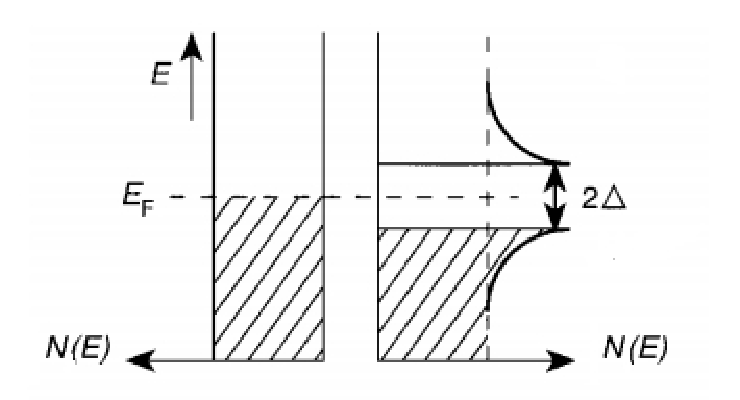
\includegraphics[width=0.3\textwidth]{img/f1.pdf}}
\caption*{\textbf{Figure 2: }\small \textbf{(a)} Phase Transitions in the T-B-diagram. \textbf{(b)} Meißner-Ochsenfeld Effect. \textbf{(c)} Phenomenological sketch of electron-electron interaction leading to cooper pairs. \textbf{(d)} Density of states in a regular conductor (left) and a supercoductor (right) \cite{buckel}.}
\label{fig:tb}
\end{figure}


\ssubsection{BCS Theory}
To understand how the electrons behave in very cold materials one has to include the movement of the nuclei. Unlike high temperature theories, that can ignore these movements (Born Oppenheim approximation), they now happen on the same timescale as the movement of electrons. Consider for simplicities sake a single electron in a regular lattice. The surrounding nuclei are accelerated towards this electron and due to inertia will continue moving in this direction, even as the electron moves on. This retarded aggregation of positive nuclei creates a positive pseudo charge behind the electron which in turn attracts other electrons (cf. figure 2c). By mechanism of lattice deformations ($\rightarrow$ phonons) a new (attractive) electron-electron interaction has to be considered, that can even create bound states: cooper pairs. These cooper pairs now have a total spin of 0 and act as bosons, allowing them to occupy the same conducting state several times without interfering. Thus the material becomes super conducting.

Even though this is only a rough classical explanation of a sub quantum mechanical phenomenon, it can already describe a lot of experimentally observed effects: high energies induced by currents, magnetic fields or high temperatures destroy the super conductance (by destroying the cooper pairs). Furthermore different isotopes have different critical temperatures (due to the different inertia).

\ssubsection{Statistics}
A superconducting material is in neither a pure Fermi nor Bose state. Only about 10\% of all electrons form cooper pairs and can occupy already filled states. The density of states thus still resembles that of a Fermi state (e.g. free electron gas). The cooper pairs that do exist are created near the Fermi energy as they require an intermediate free state to form a pair. Considering the limited lifetime of the pairs, the resulting density of states is only changed near the Fermi energy like in figure 2d with a small energy gap corresponding to the energy required to form a cooper pair and an increased density of states just below.

\ssubsection{Experiment} 
The critical temperature and the critical magnetic field of tin and indium can be measured using the property of vanishing magnetic permeability in the superconducting phase. The permeability is measured using an electronic circuit similar to a transformer. A second induction system operated at the same voltage is used as a reference system. The whole setup is placed within an cryogenic chamber, build by two vacuum separated and silvered cryostats. The outer dewar is filled with liquid nitrogen and the inner one with liquid helium. The pressure of the helium is tunable with a pump and is used to regulate the temperature measured through the vapor pressure. A long coil is used to generate an external magnetic field.

\ssubsection{References}
\vspace*{-1cm}
\nocite{buckel}
\nocite{tinkham}
\nocite{BCS}
\nocite{GL}
\nocite{hofmann}
\renewcommand\refname{}
\bibliographystyle{unsrt}
\bibliography{bib}

\end{document}
